%%%%%%%%%%%% 付録 %%%%%%%%%%%%%%%%
%\chapter{一般化確率ペトリネット(GSPN)の解説}{\label{sec:app}}
%本章では,本文中に出てくる一般化確率ペトリネット(GSPN)について解説する.
%まず,Petri Net(PN)とはプレースとトランジションと呼ばれる2種類のノードを持つ有効二部グラフとして表現され,離散事象を効率よくモデル化するためのモデリング言語として用いられる.
%PNはプレース(白丸),トランジション(長方形),トークン(黒丸)の3項組で構成され,トランジションの発火でプレース内のトークンが移動する.
%PNでは,全プレースに対するトークンの状態(マーキング)によってシステムの動作を記述する.
%図 \ref{fig:2-1}のt1の様に,トランジションの入力に対するプレースにトークンが存在するとき,そのトランジションは発火可能といい,トランジションの発火により入力に対するプレース内のトークンが出力に対するプレースに移動する.
%発火後のペトリネットが図 \ref{fig:2-2}である.
%トランジションが発火可能になってから実際に発火するまでのタイミングや発火可能なマーキングを設定することで様々なシステムのモデリングを行うことができる.
%
%PNはトランジションの発火タイミングにより分類される.
%一般に,発火遅延が指数分布に従うトランジションで構成されるPNは確率ペトリネット(Stochastic Petri Net; SPN)と呼ばれており,その中でも瞬時トランジションを部分的に許容するものを一般確率ペトリネット(Generalized Stochastic Petri Net; GSPN)と呼ぶ.
%
%本論文のペトリネット図においてプレースは白丸,指数トランジションは実線の長方形,瞬時トランジションは点線の長方形で表されている.
%また,解析方法としてはJSPetirNet \cite{siryo2} という広島大学で開発されたPN解析ツールを利用してペトリネットのマーキングの生成,グループ化,解析のための行列作成を行い,作成された行列をrubyのスクリプトにより,Rで利用する連続時間マルコフ連鎖の遷移行列に変換した後に,Rを用いて連続時間マルコフ連鎖の定常解析を行った.

\chapter{Detail of Generalized Stochastic Petri Net (GSPN)}{\label{sec:app}}
In this chapter, we will explain the generalized Stochastic Petri Net (GSPN) used in the main text.
First, Petri Net (PN) is expressed as a directed bipartite graph with two kinds of nodes called places and transitions, and it is used as a modeling language for modeling discrete events efficiently.
The PN consists of 3 tuples of places (open circles), transitions (rectangles), and tokens (filled circles).
The tokens in the place move as the transition fires.
In the PN, the behavior of the system is described by the state of the token (marking) for all places.
When a token exists in the place for the input of the trasition like t1 of figure \ref{fig:2-1}, the trasition's state is called "can fire", and by firing, the token in the input place is moved to output place.
The PN after the t1 fired is shown at figure  \ref{fig:2-2}.
Modeling of various systems can be done by setting the timing for when for when the trasition fires from when it get to the state "can fire" and by setting the ignitable marking.

PN is categorized according to transition firing timing.
In general, PNs composed of transitions whose firing delay follow the exponential distribution are called Stochastic Petri Net (SPN), and among them, those that allow instant transitions partially are called Generalized Stochastic Petri Net (GSPN).

In the PN diagram of this paper, places are represented by white circles, exponential transitions are represented by rectangles with solid lines, and instant transitions are represented by rectangles with dotted lines.
As a method of analysis, we created a matrix for generating, grouping and analyszeing Petri Net marking using PN analysis tool developed at Hiroshima University called JSPetriNet \cite{siryo2}.
Then using Ruby's script, we convert the matrix to the transition matrix of continuous-time Markov chain (CTMC) that can be used in R.
At last, we did steady state analysis of CTMC using R.


\begin{figure}[p]
\begin{center}
	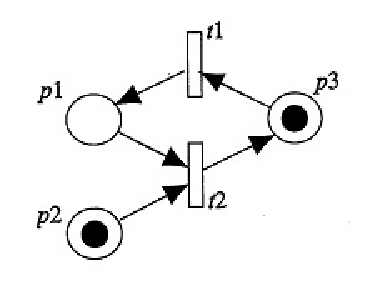
\includegraphics[]{fig/2-1.eps}
\end{center}
\caption{Petri Net with t1 "can fire"}
\label{fig:2-1}
\end{figure}


\begin{figure}[p]
\begin{center}
	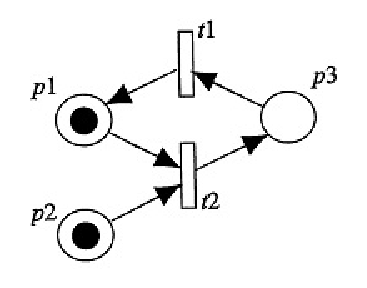
\includegraphics[]{fig/2-2.eps}
\end{center}
\caption{Petri Net after t1 fired}
\label{fig:2-2}
\end{figure}

\setlength{\columnseprule}{0.4pt}
\chapter{Source code of GSPN}
%ここでは本文で紹介したペトリネットに対応する,JSPetriNetにおけるペトリネット生成に使用したソースコードを紹介する.
Here we introduce the source code used for Petri Net generation in JSPetriNet, corresponding to thePetri Net introduced in the main text.

\section{Source code of figure \ref{fig:original}}
\begin{figure}[ht]
\begin{small}
\begin{verbatim}
place Pa
place Pb
place Pca
place Pcb
place Pd
place Pe
place Pfd
place Pfe


exp a (guard = ga)
exp b (guard = gb)
exp ca (guard = gca)
exp cb (guard = gcb)
exp c (guard = gc)
exp fd (guard =gfd)
exp fe (guard = gfe)
exp f


arc a to Pa
arc b to Pb
arc Pa to ca
arc Pb to cb
arc ca to Pca
arc cb to Pcb
arc Pca to c
arc Pcb to c
\end{verbatim}
\end{small}
\end{figure}

\begin{figure}[ht]
\begin{small}
\begin{verbatim}
arc c to Pd
arc c to Pe
arc Pd to fd
arc Pe to fe
arc fd to Pfd
arc fe to Pfe
arc Pfd to f
arc Pfe to f


na = 2
nb = 2
nca = 3
ncb = 3
nd = 2
ne = 2
nfd = 3
nfe = 3

ga := #Pa < na
gb := #Pb < nb
gca := #Pca < nca
gcb := #Pcb < ncb
gc := #Pd < nd && #Pe < ne
gfd := #Pfd < nfd
gfe := #Pfe < nfe

rwd.f := ifelse(#Pfd >= 1 && #Pfe >= 1, 1, 0)
rwd.ablock := ifelse(#Pa==2, 1, 0)
rwd.cablock := ifelse(#Pca==3, 1, 0)
rwd.cblock := ifelse(#Pd==2 || #Pe==2, 1, 0)
rwd.dblock := ifelse(#Pfd==3, 1, 0)

\end{verbatim}
\end{small}
\end{figure}

\clearpage

\section{Source code of figure \ref{fig:FFSo}}
\begin{figure}[ht]
\begin{small}
\begin{verbatim}
place Pa
place Pb
place Pca
place Pcb
place Pd
place Pe

place Pfd1f
place Pfd2f
place Pfd3f
place Pfd1t
place Pfd2t
place Pfd3t
place Pfe1f
place Pfe2f
place Pfe3f
place Pfe1t
place Pfe2t
place Pfe3t


exp a (guard = ga)
exp b (guard = gb)

exp ca (guard = gca)
exp cafail (guard = gca)

exp cb (guard = gcb)
exp cbfail (guard = gcb)

exp c (guard = gc)
exp cfail (guard = gc)

exp df (guard = gd1)
exp dt (guard = gd1)
imm df2 (guard = gd2)
imm dt2 (guard = gd2)
imm df3 (guard = gd3)
imm dt3 (guard = gd3)
\end{verbatim}
\end{small}
\end{figure}
\begin{figure}[ht]
\begin{small}
\begin{verbatim}
exp ef (guard = ge1)
exp et (guard = ge1)
imm ef2 (guard = ge2)
imm et2 (guard = ge2)
imm ef3 (guard = ge3)
imm et3 (guard = ge3)

imm f1
imm f2
imm f3
exp f4
exp f4fail

arc a to Pa
arc b to Pb

arc Pa to ca
arc Pa to cafail

arc Pb to cb
arc Pb to cbfail

arc ca to Pca
arc cb to Pcb

arc Pca to c
arc Pcb to c
arc Pca to cfail
arc Pcb to cfail

arc c to Pd
arc c to Pe

arc Pd to df
arc Pd to dt

arc df to Pfd1f
arc Pfd1f to df2
arc df2 to Pfd2f
arc Pfd2f to df3
arc df3 to Pfd3f

arc dt to Pfd1t
arc Pfd1t to dt2
arc dt2 to Pfd2t
arc Pfd2t to dt3
arc dt3 to Pfd3t

arc Pe to ef
arc Pe to et

\end{verbatim}
\end{small}
\end{figure}
\begin{figure}[ht]
\begin{small}
\begin{verbatim}

arc ef to Pfe1f
arc Pfe1f to ef2
arc ef2 to Pfe2f
arc Pfe2f to ef3
arc ef3 to Pfe3f

arc et to Pfe1t
arc Pfe1t to et2
arc et2 to Pfe2t
arc Pfe2t to et3
arc et3 to Pfe3t

arc Pfd3f to f1
arc Pfe3f to f1
arc Pfd3t to f2
arc Pfe3f to f2
arc Pfd3f to f3
arc Pfe3t to f3

arc Pfd3t to f4
arc Pfe3t to f4
arc Pfd3t to f4fail
arc Pfe3t to f4fail

ga := #Pa < 2
gb := #Pb < 2
gca := #Pca < 3
gcb := #Pcb < 3
gc := #Pd < 2 && #Pe < 2

gd1 := #Pfd1f == 0 && #Pfd1t == 0
gd2 := #Pfd2f == 0 && #Pfd2t == 0
gd3 := #Pfd3f == 0 && #Pfd3t == 0
ge1 := #Pfe1f == 0 && #Pfe1t == 0
ge2 := #Pfe2f == 0 && #Pfe2t == 0
ge3 := #Pfe3f == 0 && #Pfe3t == 0

rwd.f := ifelse(?f4, f4.rate, 0)
rwd.ablock := ifelse(#Pa == 2, 1,0)
rwd.cablock := ifelse(#Pca==3, 1, 0)
rwd.cblock := ifelse(#Pd==2 || #Pe==2, 1, 0)
rwd.dblock := ifelse(#Pfd1f == 1 || #Pfd1t == 1, 1, 0)

\end{verbatim}
\label{fig:FFSospn}
\end{small}
\end{figure}

\clearpage

\section{Source code of figure \ref{fig:FFSx}}
\begin{figure}[ht]
\begin{small}
\begin{verbatim}
place Pa
place Pb
place Pca
place Pcb
place Pd
place Pe

place Pfd1f
place Pfd2f
place Pfd3f
place Pfd1t
place Pfd2t
place Pfd3t
place Pfe1f
place Pfe2f
place Pfe3f
place Pfe1t
place Pfe2t
place Pfe3t

exp a (guard = ga)

exp b (guard = gb)

exp ca (guard = gca)
exp cafail (guard = gca)

exp cb (guard = gcb)
exp cbfail (guard = gcb)

exp c (guard = gc)
exp cfail (guard = gc)

exp df (guard = gd1)
exp dt (guard = gd1)
imm df2 (guard = gd2, priority=1)
imm dt2 (guard = gd2, priority=1)
imm df3 (guard = gd3, priority=1)
imm dt3 (guard = gd3, priority=1)

\end{verbatim}
\end{small}
\end{figure}

\begin{figure}[ht]
\begin{small}
\begin{verbatim}

exp ef (guard = ge1)
exp et (guard = ge1)
imm ef2 (guard = ge2, priority=1)
imm et2 (guard = ge2, priority=1)
imm ef3 (guard = ge3, priority=1)
imm et3 (guard = ge3, priority=1)

imm f1
imm f2
exp f4
exp f4fail

imm deadd (guard = gdeadd)
imm deade (guard = gdeade)

arc a to Pa
arc b to Pb

arc Pa to ca
arc Pa to cafail

arc Pb to cb
arc Pb to cbfail

arc ca to Pca
arc cb to Pcb

arc Pca to c
arc Pcb to c
arc Pca to cfail
arc Pcb to cfail

arc c to Pd
arc c to Pe

arc Pd to df
arc Pd to dt

arc df to Pfd1f
arc Pfd1f to df2
arc df2 to Pfd2f
arc Pfd2f to df3
arc df3 to Pfd3f

arc dt to Pfd1t
arc Pfd1t to dt2
arc dt2 to Pfd2t
arc Pfd2t to dt3
arc dt3 to Pfd3t

arc Pe to ef
arc Pe to et

arc ef to Pfe1f
arc Pfe1f to ef2
arc ef2 to Pfe2f
arc Pfe2f to ef3
arc ef3 to Pfe3f
\end{verbatim}
\end{small}
\end{figure}

\begin{figure}[ht]
\begin{small}
\begin{verbatim}
arc et to Pfe1t
arc Pfe1t to et2
arc et2 to Pfe2t
arc Pfe2t to et3
arc et3 to Pfe3t

arc Pfd3f to f1
arc Pfe3f to f2

arc Pfd3t to f4
arc Pfe3t to f4
arc Pfd3t to f4fail
arc Pfe3t to f4fail

arc Pfd3t to deadd
arc Pfe3t to deade

ga := #Pa < 2
gb := #Pb < 2
gca := #Pca < 3
gcb := #Pcb < 3
gc := #Pd < 2 && #Pe < 2

gd1 := #Pfd1f == 0 && #Pfd1t == 0
gd2 := #Pfd2f == 0 && #Pfd2t == 0
gd3 := #Pfd3f == 0 && #Pfd3t == 0
ge1 := #Pfe1f == 0 && #Pfe1t == 0
ge2 := #Pfe2f == 0 && #Pfe2t == 0
ge3 := #Pfe3f == 0 && #Pfe3t == 0

gdeade := #Pa == 2 && #Pb == 2 && #Pca == 3 && #Pcb == 3 && #Pe == 2 && (#Pfe1t == 1 || #Pfe1f == 1) &&
          (#Pfe2t == 1 || #Pfe2f == 1) && (#Pfe3t == 1 || #Pfe3f == 1) && #Pd == 0 && #Pfd1t == 0 &&
           #Pfd2t == 0 && #Pfd3t == 0
gdeadd := #Pa == 2 && #Pb == 2 && #Pca == 3 && #Pcb == 3 && #Pe == 0 && #Pfe1t == 0 && #Pfe2t == 0 &&
           #Pfe3t == 0 && #Pd == 2 && (#Pfd1t == 1 || #Pfd1f == 1) && (#Pfd2t == 1 || #Pfd2f == 1) &&
           (#Pfd3t == 1 || #Pfd3f == 1)

rwd.f := ifelse(?f4, f4.rate, 0)
rwd.ablock := ifelse(#Pa==2, 1,0)
rwd.cablock := ifelse(#Pca==3, 1, 0)
rwd.cblock := ifelse(#Pd==2 || #Pe==2, 1, 0)
rwd.dblock := ifelse(#Pfd1f==1 || #Pfd1t==1, 1, 0)

\end{verbatim}
\end{small}
\end{figure}

\clearpage

\section{Source code of figure \ref{fig:ffs4}}

\begin{figure}[ht]
\begin{small}
\begin{verbatim}
place Pa
place Pb

place Pcat1
place Pcat2
place Pcat3

place Pcaf1
place Pcaf2
place Pcaf3

place Pcbt1
place Pcbt2
place Pcbt3

place Pcbf1
place Pcbf2
place Pcbf3

place Pd1
place Pd2

place Pe1
place Pe2

place Pdf1
place Pdf12

place Pef1
place Pef12

place Pfdt1
place Pfdt2
place Pfdt3
place Pfdf1
place Pfdf2
place Pfdf3

place Pfet1
place Pfet2
place Pfet3
\end{verbatim}
\end{small}
\end{figure}

\begin{figure}[ht]
\begin{small}
\begin{verbatim}
place Pfef1
place Pfef2
place Pfef3

place Pfdf11
place Pfdf12
place Pfdf13
place Pfef11
place Pfef12
place Pfef13


exp a (guard = ga)
exp b (guard = gb)

exp ca (guard = gca1)
exp cafail(guard = gca1)
imm cat1 (guard = gca2)
imm cat2 (guard = gca3)
imm caf1 (guard = gca2)
imm caf2 (guard = gca3)

exp cb (guard = gcb1)
exp cbfail (guard = gcb1)
imm cbt1 (guard = gcb2)
imm cbt2 (guard = gcb3)
imm cbf1 (guard = gcb2)
imm cbf2 (guard = gcb3)

exp c (guard = gc)
exp cf1 (guard = gc)
exp cf2 (guard = gc)
exp cf3 (guard = gc)
exp cf4 (guard = gc)

imm d (guard = gd)
imm d1 (guard = gd)

imm e (guard = ge)
imm e1 (guard = ge)

exp dt (guard = gd1)
exp df (guard = gd1)
imm fdt1 (guard = gd2)
imm fdt2 (guard = gd3)
imm fdf1 (guard = gd2)
imm fdf2 (guard = gd3)

exp df1 (guard = gd1)
imm fdf11 (guard = gd2)
imm fdf12 (guard = gd3)

exp et (guard = ge1)
exp ef (guard = ge1)
imm fet1 (guard = ge2)
imm fet2 (guard = ge3)
imm fef1 (guard = ge2)
imm fef2 (guard = ge3)
\end{verbatim}
\end{small}
\end{figure}

\begin{figure}[ht]
\begin{small}
\begin{verbatim}
exp ef1 (guard = ge1)
imm fef11 (guard = ge2)
imm fef12 (guard = ge3)


exp f
exp ff
exp f1
exp f2
exp f3
exp ff1

arc a to Pa
arc b to Pb

arc Pa to ca
arc ca to Pcat1
arc Pcat1 to cat1
arc cat1 to Pcat2
arc Pcat2 to cat2
arc cat2 to Pcat3

arc Pa to cafail
arc cafail to Pcaf1
arc Pcaf1 to caf1
arc caf1 to Pcaf2
arc Pcaf2 to caf2
arc caf2 to Pcaf3

arc Pb to cb
arc cb to Pcbt1
arc Pcbt1 to cbt1
arc cbt1 to Pcbt2
arc Pcbt2 to cbt2
arc cbt2 to Pcbt3

arc Pb to cbfail
arc cbfail to Pcbf1
arc Pcbf1 to cbf1
arc cbf1 to Pcbf2
arc Pcbf2 to cbf2
arc cbf2 to Pcbf3


arc Pcat3 to c
arc Pcbt3 to c
arc Pcat3 to cf1
arc Pcbt3 to cf1
arc Pcaf3 to cf2
arc Pcbt3 to cf2
arc Pcat3 to cf3
arc Pcbf3 to cf3
arc Pcaf3 to cf4
arc Pcbf3 to cf4

arc c to Pd1
arc c to Pe1
arc Pd1 to d
arc d to Pd2
arc Pe1 to e
arc e to Pe2
\end{verbatim}
\end{small}
\end{figure}

\begin{figure}[ht]
\begin{small}
\begin{verbatim}
arc cf1 to Pdf1
arc cf1 to Pef1
arc Pdf1 to d1
arc d1 to Pdf12
arc Pef1 to e1
arc e1 to Pef12

arc cf2 to Pdf1
arc cf2 to Pef1

arc cf3 to Pdf1
arc cf3 to Pef1

arc cf4 to Pdf1
arc cf4 to Pef1

arc Pd2 to dt
arc Pd2 to df

arc df to Pfdf1
arc Pfdf1 to fdf1
arc fdf1 to Pfdf2
arc Pfdf2 to fdf2
arc fdf2 to Pfdf3

arc dt to Pfdt1
arc Pfdt1 to fdt1
arc fdt1 to Pfdt2
arc Pfdt2 to fdt2
arc fdt2 to Pfdt3


arc Pe2 to et
arc Pe2 to ef

arc ef to Pfef1
arc Pfef1 to fef1
arc fef1 to Pfef2
arc Pfef2 to fef2
arc fef2 to Pfef3

arc et to Pfet1
arc Pfet1 to fet1
arc fet1 to Pfet2
arc Pfet2 to fet2
arc fet2 to Pfet3


arc Pdf12 to df1
arc df1 to Pfdf11
arc Pfdf11 to fdf11
arc fdf11 to Pfdf12
arc Pfdf12 to fdf12
arc fdf12 to Pfdf13

arc Pef12 to ef1
arc ef1 to Pfef11
arc Pfef11 to fef11
arc fef11 to Pfef12
arc Pfef12 to fef12
arc fef12 to Pfef13
\end{verbatim}
\end{small}
\end{figure}

\begin{figure}[ht]
\begin{small}
\begin{verbatim}
arc Pfdf13 to ff1
arc Pfef13 to ff1


arc Pfdf3 to f1
arc Pfef3 to f1
arc Pfdt3 to f2
arc Pfef3 to f2
arc Pfdf3 to f3
arc Pfet3 to f3

arc Pfdt3 to f
arc Pfet3 to f
arc Pfdt3 to ff
arc Pfet3 to ff


ga := #Pa < 2
gb := #Pb < 2

gca1 := #Pcat1 == 0 && #Pcaf1 == 0
gca2 := #Pcat2 == 0 && #Pcaf2 == 0
gca3 := #Pcat3 == 0 && #Pcaf3 == 0

gcb1 := #Pcbt1 == 0 && #Pcbf1 == 0
gcb2 := #Pcbt2 == 0 && #Pcbf2 == 0
gcb3 := #Pcbt3 == 0 && #Pcbf3 == 0

gc := #Pd1==0 && #Pe1==0 && #Pdf1==0 && #Pef1==0
gd := #Pd2==0 && #Pdf12==0
ge := #Pe2==0 && #Pef12==0

gd1 := #Pfdf1==0 && #Pfdt1==0 && #Pfdf11==0
gd2 := #Pfdf2==0 && #Pfdt2==0 && #Pfdf12==0
gd3 := #Pfdf3==0 && #Pfdt3==0 && #Pfdf13==0

ge1 := #Pfef1==0 && #Pfet1==0 && #Pfef11==0
ge2 := #Pfef2==0 && #Pfet2==0 && #Pfef12==0
ge3 := #Pfef3==0 && #Pfet3==0 && #Pfef13==0

rwd.f := ifelse(#Pfdt3==1 && #Pfet3==1, f.rate, 0)
rwd.ablock := ifelse(#Pa==2, 1, 0)
rwd.cablock := ifelse(#Pcat1==1 || #Pcaf1==1, 1, 0)
rwd.cblock := ifelse(#Pd1==1 || #Pe1==1 || #Pdf1==1 || #Pef1==1, 1, 0)
rwd.dblock := ifelse(#Pfdt1==1 || #Pfdf1==1 || #Pfdf11==1, 1, 0)


\end{verbatim}
\end{small}
\end{figure}

\clearpage

\section{Source code of figure \ref{fig:ffs14}}
\begin{figure}[ht]
\begin{small}
\begin{verbatim}
place Pa
place Pb

place Pcat1
place Pcat2
place Pcat3

place Pcbt1
place Pcbt2
place Pcbt3

place Pd1
place Pd2

place Pe1
place Pe2

place Pdf1
place Pdf12
place Pef1
place Pef12

place Pfdt1
place Pfdt2
place Pfdt3
place Pfdf1
place Pfdf2
place Pfdf3

place Pfet1
place Pfet2
place Pfet3
place Pfef1
place Pfef2
place Pfef3

place Pfdf11
place Pfdf12
place Pfdf13
\end{verbatim}
\end{small}
\end{figure}

\begin{figure}[ht]
\begin{small}
\begin{verbatim}
place Pfef11
place Pfef12
place Pfef13


exp a (guard = ga)
exp b (guard = gb)

exp ca (guard = gca1)
exp cafail(guard = gca1)
imm cat1 (guard = gca2)
imm cat2 (guard = gca3)

exp cb (guard = gcb1)
exp cbfail (guard = gcb1)
imm cbt1 (guard = gcb2)
imm cbt2 (guard = gcb3)

exp c (guard = gc)
exp cf1 (guard = gc)

imm d (guard = gd)
imm d1 (guard = gd)

imm e (guard = ge)
imm e1 (guard = ge)

exp dt (guard = gd1)
exp df (guard = gd1)
imm fdt1 (guard = gd2)
imm fdt2 (guard = gd3)
imm fdf1 (guard = gd2)
imm fdf2 (guard = gd3)

exp et (guard = ge1)
exp ef (guard = ge1)
imm fet1 (guard = ge2)
imm fet2 (guard = ge3)
imm fef1 (guard = ge2)
imm fef2 (guard = ge3)

exp df1 (guard = gd1)
imm fdf11 (guard = gd2)
imm fdf12 (guard = gd3)

exp ef1 (guard = ge1)
imm fef11 (guard = ge2)
imm fef12 (guard = ge3)

exp f
exp ff
exp f1
exp f2
exp f3
exp ff1


arc a to Pa
arc b to Pb
\end{verbatim}
\end{small}
\end{figure}

\begin{figure}[ht]
\begin{small}
\begin{verbatim}
arc Pa to ca
arc ca to Pcat1
arc Pcat1 to cat1
arc cat1 to Pcat2
arc Pcat2 to cat2
arc cat2 to Pcat3

arc Pb to cb
arc cb to Pcbt1
arc Pcbt1 to cbt1
arc cbt1 to Pcbt2
arc Pcbt2 to cbt2
arc cbt2 to Pcbt3

arc Pa to cafail
arc Pb to cbfail

arc Pcat3 to c
arc Pcbt3 to c
arc Pcat3 to cf1
arc Pcbt3 to cf1

arc c to Pd1
arc c to Pe1
arc Pd1 to d
arc d to Pd2
arc Pe1 to e
arc e to Pe2

arc cf1 to Pdf1
arc cf1 to Pef1
arc Pdf1 to d1
arc d1 to Pdf12
arc Pef1 to e1
arc e1 to Pef12

arc Pd2 to dt
arc Pd2 to df

arc df to Pfdf1
arc Pfdf1 to fdf1
arc fdf1 to Pfdf2
arc Pfdf2 to fdf2
arc fdf2 to Pfdf3

arc dt to Pfdt1
arc Pfdt1 to fdt1
arc fdt1 to Pfdt2
arc Pfdt2 to fdt2
arc fdt2 to Pfdt3


arc Pe2 to et
arc Pe2 to ef

arc ef to Pfef1
arc Pfef1 to fef1
arc fef1 to Pfef2
arc Pfef2 to fef2
arc fef2 to Pfef3
\end{verbatim}
\end{small}
\end{figure}

\begin{figure}[ht]
\begin{small}
\begin{verbatim}
arc et to Pfet1
arc Pfet1 to fet1
arc fet1 to Pfet2
arc Pfet2 to fet2
arc fet2 to Pfet3

arc Pdf12 to df1
arc df1 to Pfdf11
arc Pfdf11 to fdf11
arc fdf11 to Pfdf12
arc Pfdf12 to fdf12
arc fdf12 to Pfdf13

arc Pef12 to ef1
arc ef1 to Pfef11
arc Pfef11 to fef11
arc fef11 to Pfef12
arc Pfef12 to fef12
arc fef12 to Pfef13

arc Pfdf13 to ff1
arc Pfef13 to ff1

arc Pfdf3 to f1
arc Pfef3 to f1
arc Pfdt3 to f2
arc Pfef3 to f2
arc Pfdf3 to f3
arc Pfet3 to f3

arc Pfdt3 to f
arc Pfet3 to f
arc Pfdt3 to ff
arc Pfet3 to ff


ga := #Pa < 2
gb := #Pb < 2

gca1 := #Pcat1 == 0
gca2 := #Pcat2 == 0
gca3 := #Pcat3 == 0

gcb1 := #Pcbt1 == 0
gcb2 := #Pcbt2 == 0
gcb3 := #Pcbt3 == 0

gc := #Pd1==0 && #Pe1==0 && #Pdf1==0 && #Pef1==0
gd := #Pd2==0 && #Pdf12==0
ge := #Pe2==0 && #Pef12==0

gd1 := #Pfdf1==0 && #Pfdt1==0 && #Pfdf11==0
gd2 := #Pfdf2==0 && #Pfdt2==0 && #Pfdf12==0
gd3 := #Pfdf3==0 && #Pfdt3==0 && #Pfdf13==0

ge1 := #Pfef1==0 && #Pfet1==0 && #Pfef11==0
ge2 := #Pfef2==0 && #Pfet2==0 && #Pfef12==0
ge3 := #Pfef3==0 && #Pfet3==0 && #Pfef13==0

rwd.f := ifelse(#Pfdt3==1 && #Pfet3==1, f.rate, 0)
rwd.ablock := ifelse(#Pa == 2, a.rate, 0)
rwd.cablock := ifelse(#Pcat1==1, 1, 0)
rwd.cblock := ifelse(#Pd1==1 || #Pe1==1 || #Pdf1==1 || #Pef1==1, 1, 0)
rwd.dblock := ifelse(#Pfdf1==1 || #Pfdt1==1 || #Pfef11==1, 1, 0)
\end{verbatim}
\end{small}
\end{figure}

\clearpage

\section{Source code of figure \ref{fig:ffs24}}
\begin{figure}[ht]
\begin{small}
\begin{verbatim}
place Pa
place Pb

place Pcat1
place Pcat2
place Pcat3

place Pcaf1
place Pcaf2
place Pcaf3

place Pcbt1
place Pcbt2
place Pcbt3
place Pcbf1
place Pcbf2
place Pcbf3

place Pd1
place Pd2

place Pe1
place Pe2

place Pfdt1
place Pfdt2
place Pfdt3
place Pfdf1
place Pfdf2
place Pfdf3

place Pfet1
place Pfet2
place Pfet3
\end{verbatim}
\end{small}
\end{figure}

\begin{figure}[ht]
\begin{small}
\begin{verbatim}
place Pfef1
place Pfef2
place Pfef3


exp a (guard = ga)
exp b (guard = gb)

exp ca (guard = gca1)
exp cafail(guard = gca1)
imm cat1 (guard = gca2)
imm cat2 (guard = gca3)
imm caf1 (guard = gca2)
imm caf2 (guard = gca3)

exp cb (guard = gcb1)
exp cbfail (guard = gcb1)
imm cbt1 (guard = gcb2)
imm cbt2 (guard = gcb3)
imm cbf1 (guard = gcb2)
imm cbf2 (guard = gcb3)

exp c (guard = gc)
exp cf1 (guard = gc)
exp cf2 (guard = gc)
exp cf3 (guard = gc)
exp cf4 (guard = gc)

imm d (guard = gd)
imm e (guard = ge)

exp dt (guard = gd1)
exp df (guard = gd1)
imm fdt1 (guard = gd2)
imm fdt2 (guard = gd3)
imm fdf1 (guard = gd2)
imm fdf2 (guard = gd3)

exp et (guard = ge1)
exp ef (guard = ge1)
imm fet1 (guard = ge2)
imm fet2 (guard = ge3)
imm fef1 (guard = ge2)
imm fef2 (guard = ge3)

exp f
exp ff
exp f1
exp f2
exp f3


arc a to Pa
arc b to Pb

arc Pa to ca
arc ca to Pcat1
arc Pcat1 to cat1
arc cat1 to Pcat2
arc Pcat2 to cat2
arc cat2 to Pcat3
\end{verbatim}
\end{small}
\end{figure}

\begin{figure}[ht]
\begin{small}
\begin{verbatim}
arc Pa to cafail
arc cafail to Pcaf1
arc Pcaf1 to caf1
arc caf1 to Pcaf2
arc Pcaf2 to caf2
arc caf2 to Pcaf3

arc Pb to cb
arc cb to Pcbt1
arc Pcbt1 to cbt1
arc cbt1 to Pcbt2
arc Pcbt2 to cbt2
arc cbt2 to Pcbt3

arc Pb to cbfail
arc cbfail to Pcbf1
arc Pcbf1 to cbf1
arc cbf1 to Pcbf2
arc Pcbf2 to cbf2
arc cbf2 to Pcbf3

arc Pcat3 to c
arc Pcbt3 to c
arc Pcat3 to cf1
arc Pcbt3 to cf1
arc Pcaf3 to cf2
arc Pcbt3 to cf2
arc Pcat3 to cf3
arc Pcbf3 to cf3
arc Pcaf3 to cf4
arc Pcbf3 to cf4

arc c to Pd1
arc c to Pe1
arc Pd1 to d
arc d to Pd2
arc Pe1 to e
arc e to Pe2

arc Pd2 to dt
arc Pd2 to df

arc df to Pfdf1
arc Pfdf1 to fdf1
arc fdf1 to Pfdf2
arc Pfdf2 to fdf2
arc fdf2 to Pfdf3

arc dt to Pfdt1
arc Pfdt1 to fdt1
arc fdt1 to Pfdt2
arc Pfdt2 to fdt2
arc fdt2 to Pfdt3

arc Pe2 to et
arc Pe2 to ef

arc ef to Pfef1
arc Pfef1 to fef1
arc fef1 to Pfef2
arc Pfef2 to fef2
arc fef2 to Pfef3
\end{verbatim}
\end{small}
\end{figure}

\begin{figure}[ht]
\begin{small}
\begin{verbatim}
arc et to Pfet1
arc Pfet1 to fet1
arc fet1 to Pfet2
arc Pfet2 to fet2
arc fet2 to Pfet3

arc Pfdf3 to f1
arc Pfef3 to f1
arc Pfdt3 to f2
arc Pfef3 to f2
arc Pfdf3 to f3
arc Pfet3 to f3

arc Pfdt3 to f
arc Pfet3 to f
arc Pfdt3 to ff
arc Pfet3 to ff


ga := #Pa < 2
gb := #Pb < 2

gca1 := #Pcat1 == 0 && #Pcaf1 == 0
gca2 := #Pcat2 == 0 && #Pcaf2 == 0
gca3 := #Pcat3 == 0 && #Pcaf3 == 0

gcb1 := #Pcbt1 == 0 && #Pcbf1 == 0
gcb2 := #Pcbt2 == 0 && #Pcbf2 == 0
gcb3 := #Pcbt3 == 0 && #Pcbf3 == 0

gc := #Pd1==0 && #Pe1==0
gd := #Pd2==0
ge := #Pe2==0

gd1 := #Pfdf1==0 && #Pfdt1==0
gd2 := #Pfdf2==0 && #Pfdt2==0
gd3 := #Pfdf3==0 && #Pfdt3==0

ge1 := #Pfef1==0 && #Pfet1==0
ge2 := #Pfef2==0 && #Pfet2==0
ge3 := #Pfef3==0 && #Pfet3==0

rwd.f := ifelse(#Pfdt3==1 && #Pfet3==1, f.rate, 0)
rwd.ablock := ifelse(#Pa == 2, a.rate, 0)
rwd.cablock := ifelse(#Pcat1==1 || #Pcaf1==1, 1, 0)
rwd.cblock := ifelse(#Pd1==1 || #Pe1==1, 1, 0)
rwd.dblock := ifelse(#Pfdf1==1 || #Pfdt1==1, 1, 0)
\end{verbatim}
\end{small}
\end{figure}
\clearpage

\section{Source code of figure \ref{fig:ffs34}}
\begin{figure}[ht]
\begin{small}
\begin{verbatim}
place Pa
place Pb

place Pcat1
place Pcat2
place Pcat3

place Pcaf1
place Pcaf2
place Pcaf3

place Pcbt1
place Pcbt2
place Pcbt3

place Pcbf1
place Pcbf2
place Pcbf3

place Pd1
place Pd2

place Pe1
place Pe2

place Pdf1
place Pdf12

place Pef1
place Pef12

place Pfdt1
place Pfdt2
place Pfdt3
place Pfdf1
place Pfdf2
place Pfdf3

place Pfet1
place Pfet2
place Pfet3
\end{verbatim}
\end{small}
\end{figure}

\begin{figure}[ht]
\begin{small}
\begin{verbatim}
place Pfef1
place Pfef2
place Pfef3

place Pfdf11
place Pfdf12
place Pfdf13
place Pfef11
place Pfef12
place Pfef13


exp a (guard = ga)
exp b (guard = gb)

exp ca (guard = gca1)
exp cafail(guard = gca1)
imm cat1 (guard = gca2)
imm cat2 (guard = gca3)
imm caf1 (guard = gca2)
imm caf2 (guard = gca3)

exp cb (guard = gcb1)
exp cbfail (guard = gcb1)
imm cbt1 (guard = gcb2)
imm cbt2 (guard = gcb3)
imm cbf1 (guard = gcb2)
imm cbf2 (guard = gcb3)

exp c (guard = gc)
exp cf1 (guard = gc)
exp cf2 (guard = gc)
exp cf3 (guard = gc)
exp cf4 (guard = gc)

imm d (guard = gd)
imm d1 (guard = gd)

imm e (guard = ge)
imm e1 (guard = ge)

exp dt (guard = gd1)
exp df (guard = gd1)
imm fdt1 (guard = gd2, priority = 1)
imm fdt2 (guard = gd3, priority = 1)
imm fdf1 (guard = gd2, priority = 1)
imm fdf2 (guard = gd3, priority = 1)

exp df1 (guard = gd1)
imm fdf11 (guard = gd2)
imm fdf12 (guard = gd3)

exp et (guard = ge1)
exp ef (guard = ge1)
imm fet1 (guard = ge2, priority = 1)
imm fet2 (guard = ge3, priority = 1)
imm fef1 (guard = ge2, priority = 1)
imm fef2 (guard = ge3, priority = 1)
\end{verbatim}
\end{small}
\end{figure}

\begin{figure}[ht]
\begin{small}
\begin{verbatim}
exp ef1 (guard = ge1)
imm fef11 (guard = ge2)
imm fef12 (guard = ge3)

imm mf1
imm mf12
imm mf13

imm mf2
imm mf22
imm mf23

imm mff1
imm mff2

exp f
exp ff
imm f1
imm f2
imm f3
imm ff1


arc a to Pa
arc b to Pb

arc Pa to ca
arc ca to Pcat1
arc Pcat1 to cat1
arc cat1 to Pcat2
arc Pcat2 to cat2
arc cat2 to Pcat3

arc Pa to cafail
arc cafail to Pcaf1
arc Pcaf1 to caf1
arc caf1 to Pcaf2
arc Pcaf2 to caf2
arc caf2 to Pcaf3

arc Pb to cb
arc cb to Pcbt1
arc Pcbt1 to cbt1
arc cbt1 to Pcbt2
arc Pcbt2 to cbt2
arc cbt2 to Pcbt3

arc Pb to cbfail
arc cbfail to Pcbf1
arc Pcbf1 to cbf1
arc cbf1 to Pcbf2
arc Pcbf2 to cbf2
arc cbf2 to Pcbf3


arc Pcat3 to c
arc Pcbt3 to c
arc Pcat3 to cf1
arc Pcbt3 to cf1
arc Pcaf3 to cf2
arc Pcbt3 to cf2
\end{verbatim}
\end{small}
\end{figure}

\begin{figure}[ht]
\begin{small}
\begin{verbatim}
arc Pcat3 to cf3
arc Pcbf3 to cf3
arc Pcaf3 to cf4
arc Pcbf3 to cf4

arc c to Pd1
arc c to Pe1
arc Pd1 to d
arc d to Pd2
arc Pe1 to e
arc e to Pe2

arc cf1 to Pdf1
arc cf1 to Pef1
arc Pdf1 to d1
arc d1 to Pdf12
arc Pef1 to e1
arc e1 to Pef12

arc cf2 to Pdf1
arc cf2 to Pef1

arc cf3 to Pdf1
arc cf3 to Pef1

arc cf4 to Pdf1
arc cf4 to Pef1

arc Pd2 to dt
arc Pd2 to df

arc df to Pfdf1
arc Pfdf1 to fdf1
arc fdf1 to Pfdf2
arc Pfdf2 to fdf2
arc fdf2 to Pfdf3

arc dt to Pfdt1
arc Pfdt1 to fdt1
arc fdt1 to Pfdt2
arc Pfdt2 to fdt2
arc fdt2 to Pfdt3


arc Pe2 to et
arc Pe2 to ef

arc ef to Pfef1
arc Pfef1 to fef1
arc fef1 to Pfef2
arc Pfef2 to fef2
arc fef2 to Pfef3

arc et to Pfet1
arc Pfet1 to fet1
arc fet1 to Pfet2
arc Pfet2 to fet2
arc fet2 to Pfet3
\end{verbatim}
\end{small}
\end{figure}

\begin{figure}[ht]
\begin{small}
\begin{verbatim}
arc Pfdt1 to mf1
arc Pfef1 to mf1
arc Pfdf1 to mf12
arc Pfet1 to mf12
arc Pfdf1 to mf13
arc Pfef1 to mf13

arc Pfdt2 to mf2
arc Pfef2 to mf2
arc Pfdf2 to mf22
arc Pfet2 to mf22
arc Pfdf2 to mf23
arc Pfef2 to mf23


arc Pdf12 to df1
arc df1 to Pfdf11
arc Pfdf11 to fdf11
arc fdf11 to Pfdf12
arc Pfdf12 to fdf12
arc fdf12 to Pfdf13

arc Pef12 to ef1
arc ef1 to Pfef11
arc Pfef11 to fef11
arc fef11 to Pfef12
arc Pfef12 to fef12
arc fef12 to Pfef13

arc Pfdf13 to ff1
arc Pfef13 to ff1

arc Pfdf11 to mff1
arc Pfef11 to mff1
arc Pfdf12 to mff2
arc Pfef12 to mff2

arc Pfdf3 to f1
arc Pfef3 to f1
arc Pfdt3 to f2
arc Pfef3 to f2
arc Pfdf3 to f3
arc Pfet3 to f3

arc Pfdt3 to f
arc Pfet3 to f
arc Pfdt3 to ff
arc Pfet3 to ff


ga := #Pa < 2
gb := #Pb < 2

gca1 := #Pcat1 == 0 && #Pcaf1 == 0
gca2 := #Pcat2 == 0 && #Pcaf2 == 0
gca3 := #Pcat3 == 0 && #Pcaf3 == 0
\end{verbatim}
\end{small}
\end{figure}

\begin{figure}[tp]
\begin{small}
\begin{verbatim}
gcb1 := #Pcbt1 == 0 && #Pcbf1 == 0
gcb2 := #Pcbt2 == 0 && #Pcbf2 == 0
gcb3 := #Pcbt3 == 0 && #Pcbf3 == 0

gc := #Pd1==0 && #Pe1==0 && #Pdf1==0 && #Pef1==0
gd := #Pd2==0 && #Pdf12==0
ge := #Pe2==0 && #Pef12==0

gd1 := #Pfdf1==0 && #Pfdt1==0 && #Pfdf11==0
gd2 := #Pfdf2==0 && #Pfdt2==0 && #Pfdf12==0
gd3 := #Pfdf3==0 && #Pfdt3==0 && #Pfdf13==0

ge1 := #Pfef1==0 && #Pfet1==0 && #Pfef11==0
ge2 := #Pfef2==0 && #Pfet2==0 && #Pfef12==0
ge3 := #Pfef3==0 && #Pfet3==0 && #Pfef13==0

rwd.f := ifelse(#Pfdt3==1 && #Pfet3==1, f.rate, 0)
rwd.ablock := ifelse(#Pa==2, 1, 0)
rwd.cablock := ifelse(#Pcat1==1 || #Pcaf1==1, 1, 0)
rwd.cblock := ifelse(#Pd1==1 || #Pe1==1 || #Pdf1==1 || #Pef1==1, 1, 0)
rwd.dblock := ifelse(#Pfdt1==1 || #Pfdf1==1 || #Pfef11==1, 1, 0)

\end{verbatim}
\end{small}
\end{figure}

